\documentclass[12pt]{article}

\usepackage[utf8x]{inputenc} % Включаем поддержку UTF8  
\usepackage[russian]{babel}  % Включаем пакет для поддержки русского языка  
\usepackage{hyperref}        % Для гиперссылок

% Математика
\usepackage{amsmath,amsfonts,amssymb,amsthm,mathtools} % AMS
\usepackage{icomma}
\usepackage{mathrsfs}

\usepackage{xcolor}

% Прога
\usepackage{etoolbox}
\usepackage{listings}

\definecolor{codegreen}{rgb}{0,0.6,0}
\definecolor{codegray}{rgb}{0.5,0.5,0.5}
\definecolor{codepurple}{rgb}{0.58,0,0.82}
\definecolor{backcolour}{rgb}{0.95,0.95,0.92}

\lstdefinestyle{mystyle}{
	backgroundcolor=\color{backcolour},   
	commentstyle=\color{codegreen},
	keywordstyle=\color{magenta},
	numberstyle=\tiny\color{codegray},
	stringstyle=\color{codepurple},
	basicstyle=\ttfamily\footnotesize,
	breakatwhitespace=false,         
	breaklines=true,                 
	captionpos=b,                    
	keepspaces=true,                 
	numbers=left,                    
	numbersep=5pt,                  
	showspaces=false,                
	showstringspaces=false,
	showtabs=false,                  
	tabsize=2
}

\lstset{style=mystyle}

% Цвета
\usepackage{xcolor}

% Картинки
\usepackage{graphicx}
\graphicspath{ {./images/} }

\usepackage{tikzsymbols}

% Работа с таблицами
\usepackage{array,tabularx,tabulary,booktabs} % Дополнительная работа с таблицами
\usepackage{longtable}  % Длинные таблицы
\usepackage{multirow} % Слияние строк в таблице

% Нумерованные списки
\usepackage[shortlabels]{enumitem} % Разные лейблы

% Текст
\usepackage[normalem]{ulem}  % для зачеркивания текста

\newtheorem{property}{Свойство}
\newtheorem{consequence}{Следствие}[property]

\DeclarePairedDelimiter\abs{\lvert}{\rvert}%
\DeclarePairedDelimiter\norm{\lVert}{\rVert}%

% Swap the definition of \abs* and \norm*, so that \abs
% and \norm resizes the size of the brackets, and the 
% starred version does not.
\makeatletter
\let\oldabs\abs
\def\abs{\@ifstar{\oldabs}{\oldabs*}}
%
\let\oldnorm\norm
\def\norm{\@ifstar{\oldnorm}{\oldnorm*}}
\makeatother

\begin{document}
	
	\thispagestyle{empty}
	\begin{center}
		\textbf{ПРАВИТЕЛЬСТВО РОССИЙСКОЙ ФЕДЕРАЦИИ}
		
		\vspace{5ex}
		
		\textbf{Федеральное государственное автономное образовательное учреждение \\ высшего образования \\ <<Национальный исследовательский университет \\ <<Высшая школа экономики>>}
	\end{center}
	\vspace{5ex}
	
	\begin{center}
		Московский институт электроники и математики им. А.Н. Тихонова  
		
		\vspace{5ex}
		
		Департамент прикладной математики
		
		\vspace{10ex}
		\textbf{Отчёт \\ по лабораторной работе №7 \\ по курсу <<Алгоритмизация и программирование>> \\ Задание № 13}
		\vspace{7ex}
		
	\end{center}
	
	\begin{center} 
		\begin{tabular}{| p{0.3\linewidth}| p{0.3\linewidth}| p{0.3\linewidth}|}
			\hline	
			ФИО студента & Номер группы & Дата \\  \hline
			& & \\  
			Кейер Александр \newline Петрович & БПМ-231 & \today\\  
			& & \\  \hline		
		\end{tabular}
	\end{center}
	
	\begin{center}
		\vspace{3ex}
		
		\vfill
		
		\normalsize
		
		\textbf{Москва, 2023}
	\end{center}
	
	\newpage
	
	%---------------------------------------------------------------------------------
	
	\section*{Задание (вариант № 13)}
	
 	Написать функцию обработки строки и программу, тестирующую данную функцию. В программе должен быть предусмотрен вывод исходный строки, которая при выделении слов не должна измениться.
 	\vspace{5pt}
	\newline
	\textbf{Дана строка, содержащая от 1 до 30 слов, в каждом из которых от 1 до 10 латинских букв и/или цифр; между соседними словами-- запятая, за последним словом -- точка. Напечатать эту же последовательность слов, но удалив из нее повторные вхождения слов.}
	
	\newpage
	
	\section*{Решение 1 (аккуратно используем strtok)}
	
	\begin{lstlisting}[language=C]
	#include <stdio.h> // Input/outpu library.
	#include <string.h> // String libarary for special function: strtok, strcat etc.
	
	// Useful directives for words.
	#define maxWordsCount 30
	#define minWordsCount 1
	#define maxWordLength 10
	#define minWordLength 1
	
	// Useful directives for string.
	#define maxSLength maxWordsCount * maxWordLength
	#define minSLength minWordsCount * minWordLength
	
	// Useful directives for string tokens.
	#define separator ","
	#define endToken "."
	
	// Function validating a string.
	int isSValid(char s[maxSLength]) {
		size_t sLength = strlen(s);
		
		char* endTokenP = strstr(s, endToken);
		
		// Checking the last symbol for a dot.
		if (endTokenP != s + sLength - 1) {
			printf("The string must have no more than 300 symbols, contain only one dot and end with this dot.\n");
			return 0;
		}
		
		// Checking string length.
		if (sLength > maxSLength || sLength < minSLength) {
			printf("Incorrect string length.\n");
			return 0;
		}
		
		// Checking string for incorrect symbols.
		for (int i = 0; s[i] != '\0'; i++) {
			if (!(
			s[i] == 44
			|| s[i] == 10
			|| s[i] == 46 
			|| (s[i] >= 65 && s[i] <= 90) 
			|| (s[i] >= 97 && s[i] <= 122) 
			|| (s[i] >= 48 && s[i] <= 57)
			)) {
				printf("The string contains incorrect symbols.\n");
				return 0;
			}
		}
		
		return 1;
	}
	
	// Function reading a string from stdin.
	int sReading(char sExternal[maxSLength]) {
		printf("Please, enter correct string:\n");
		
		char s[maxSLength];
		fseek(stdin, 0, SEEK_END); // Jumped over previous stdin. We also can clear stdin here: fflush(stdin);
		fgets(s, maxSLength, stdin);
		
		s[strlen(s) - 1] = '\0'; // Remove \n symbol.
		strcpy(sExternal, s);
		
		return 0;
	}
	
	// Function printing words array.
	int printWordsArr(char wordsArr[maxWordsCount][maxWordLength], int wordsCount) {
		for (int i = 0; i < wordsCount; i++) {
			for (int j = 0; j < maxWordLength; j++) {
				if (wordsArr[i][j] == '\0') {
					break;
				}
				
				printf("%c", wordsArr[i][j]);
			}
			
			// Placing tokens correctly.
			if (i < wordsCount - 1) {
				printf(",");
			} else {
				printf(".\n");
			}
		}
		
		return 0;
	}
	
	// Function changing matrix row.
	int changeMatrixRow(char matrix[maxWordsCount][maxWordLength], int i, char row[maxWordLength]) {
		for (int j = 0; j < maxWordLength; j++) {
			matrix[i][j] = row[j];
		}
		
		return 0;
	}
	
	// Function checking for the presence of a row in array.
	int isMatrixContainRow(char matrix[maxWordsCount][maxWordLength], int rowsCount, char row[maxWordLength]) {
		for (int i = 0; i < rowsCount; i++) {
			for (int j = 0; j < maxWordLength; j++) {
				if (matrix[i][j] != row[j]) {
					break;
				}
				
				// Checking for the end token.
				if (matrix[i][j] == '\0' || j == maxWordLength - 1) {
					return 1;
				}
			}
		}
		
		return 0;
	}
	
	// Function presenting solution.
	void solution(char s[maxSLength]) {
		printf("You entered string: %s\n", s);
		
		// String validation.
		if (!isSValid(s)) {
			return;
		}
		
		s[strlen(s) - 1] = '\0'; // Remove . symbol.
		
		// Useful variables initialization.
		char* word;
		int uniqueWordsCount = 0;
		int wordsCount = 0;
		char wordsArr[maxWordsCount][maxWordLength];
		
		word = strtok(s, separator);
		
		// Checking for correctly first word.
		if (word == NULL) {
			printf("Incorrect word length or words count.\n");
			return;
		}
		
		// Splitting string into words.
		while (word != NULL) {
			size_t wordLength = strlen(word);
			
			// Checking for correctly rest words.
			if (
			wordLength < minWordLength 
			|| wordLength > maxWordLength 
			|| wordsCount > maxWordsCount
			) {
				printf("Incorrect word length or words count.\n");
				return;
			}
			
			// Adding word into special array.
			if (!isMatrixContainRow(wordsArr, uniqueWordsCount, word)) {
				changeMatrixRow(wordsArr, uniqueWordsCount++, word);
			} 
			
			wordsCount++;
			word = strtok(NULL, separator);
		}
		
		printf("New string: ");
		
		// Printing special word array.
		printWordsArr(wordsArr, uniqueWordsCount);
	}
	
	// Main function.
	int main() {
		
		// Test 1.
		printf("Test 1\n");
		char s1[] = "a,a.";
		solution(s1);
		printf("\n===\n\n");
		
		// Test 2.
		printf("Test 2\n");
		char s2[] = "a,a";
		solution(s2);
		printf("\n===\n\n");
		
		// Test 3.
		printf("Test 3\n");
		char s3[] = "a.a.";
		solution(s3);
		printf("\n===\n\n");
		
		// Test 4.
		printf("Test 4\n");
		char s4[] = ".";
		solution(s4);
		printf("\n===\n\n");
		
		// Test 5.
		printf("Test 5\n");
		char s5[] = "asdasdasdas.";
		solution(s5);
		printf("\n===\n\n");
		
		// Test 6.
		printf("Test 6\n");
		char s6[] = "a,a,a,a,a,a,a,a,a,a,a,a,a,a,a,a,a,a,a,a,a,a,a,a,a,a,a,a,a,a,a,a,a,a,a,a,a,a,a,a,a,a,a,a,a,a,a,a,a,a,a,a,a,a,a,a,a,a,a,a,a.";
		solution(s6);
		printf("\n===\n\n");
		
		// Test 7.
		printf("Test 7\n");
		char s7[] = "aaaaaaaaaaaaaaaaaaaaaaaaaaaaaaaaaaaaaaaaaa,aaaaaaaaaaaaaaaaaaaaaaaaaaaaaaaaaaaaaaaaaa,aaaaaaaaaaaaaaaaaaaaaaaaaaaaaaaaaaaaaaaaaaa,aaaaaaaaaaaaaaaaaaaaaaaaaaaaaaaaaaaaaaaa,aaaaaaaaaaaaaaaaaaaaaaaaaaaaaaaaaaaaaaaaaaaaa,aaaaaaaaaaaaaaaaaaaaaaaaaaaaaaaaaaaaaaa,aaaaaaaaaaaaaaaaaaaaaaaaaaaaaaaaaaaaaaaaaaaaaaaaa.";
		solution(s7);
		printf("\n===\n\n");
		
		// User test.
		char s8[] = "";
		sReading(s8);
		solution(s8);
		
		return 0;
	}
	\end{lstlisting}
	
	\newpage
	
	\section*{Решение 2 (аккуратно не используем strtok)}
	
	\begin{lstlisting}[language=C]
	#include <stdio.h> // Input/outpu library.
	#include <string.h> // String libarary for special function: strtok, strcat etc.
	
	// Useful directives for words.
	#define maxWordsCount 30
	#define minWordsCount 1
	#define maxWordLength 10
	#define minWordLength 1
	
	// Useful directives for string.
	#define maxSLength maxWordsCount * maxWordLength
	#define minSLength minWordsCount * minWordLength
	
	// Useful directives for string tokens.
	#define separator ","
	#define endToken "."
	
	// Function validating a string.
	int isSValid(char s[maxSLength]) {
		size_t sLength = strlen(s);
		
		char* endTokenP = strstr(s, endToken);
		
		// Checking the last symbol for a dot.
		if (endTokenP != s + sLength - 1) {
			printf("The string must have no more than 300 symbols, contain only one dot and end with this dot.\n");
			return 0;
		}
		
		// Checking string length.
		if (sLength > maxSLength || sLength < minSLength) {
			printf("Incorrect string length.\n");
			return 0;
		}
		
		// Checking string for incorrect symbols.
		for (int i = 0; s[i] != '\0'; i++) {
			if (!(
			s[i] == 44
			|| s[i] == 10
			|| s[i] == 46 
			|| (s[i] >= 65 && s[i] <= 90) 
			|| (s[i] >= 97 && s[i] <= 122) 
			|| (s[i] >= 48 && s[i] <= 57)
			)) {
				printf("The string contains incorrect symbols.\n");
				return 0;
			}
		}
		
		return 1;
	}
	
	// Function reading a string from stdin.
	int sReading(char sExternal[maxSLength]) {
		printf("Please, enter correct string:\n");
		
		char s[maxSLength];
		fseek(stdin, 0, SEEK_END); // Jumped over previous stdin. We also can clear stdin here: fflush(stdin);
		fgets(s, maxSLength, stdin);
		
		s[strlen(s) - 1] = '\0'; // Remove \n symbol.
		strcpy(sExternal, s);
		
		return 0;
	}
	
	// Function printing words array.
	int printWordsArr(char wordsArr[maxWordsCount][maxWordLength], int wordsCount) {
		for (int i = 0; i < wordsCount; i++) {
			for (int j = 0; j < maxWordLength; j++) {
				if (wordsArr[i][j] == '\0') {
					break;
				}
				
				printf("%c", wordsArr[i][j]);
			}
			
			// Placing tokens correctly.
			if (i < wordsCount - 1) {
				printf(",");
			} else {
				printf(".\n");
			}
		}
		
		return 0;
	}
	
	// Function changing matrix row.
	int changeMatrixRow(char matrix[maxWordsCount][maxWordLength], int i, char row[maxWordLength]) {
		for (int j = 0; j < maxWordLength; j++) {
			matrix[i][j] = row[j];
		}
		
		return 0;
	}
	
	// Function checking for the presence of a row in array.
	int isMatrixContainRow(char matrix[maxWordsCount][maxWordLength], int rowsCount, char row[maxWordLength]) {
		for (int i = 0; i < rowsCount; i++) {
			for (int j = 0; j < maxWordLength; j++) {
				if (matrix[i][j] != row[j]) {
					break;
				}
				
				// Checking for the end token.
				if (matrix[i][j] == '\0' || j == maxWordLength - 1) {
					return 1;
				}
			}
		}
		
		return 0;
	}
	
	// Function presenting solution.
	void solution(char s[maxSLength]) {
		printf("You entered string: %s\n", s);
		
		// String validation.
		if (!isSValid(s)) {
			return;
		}
		
		s[strlen(s) - 1] = '\0'; // Remove . symbol.
		
		// Useful variables initialization.
		char word[maxWordLength] = "";
		int uniqueWordsCount = 0;
		int wordsCount = 0;
		char wordsArr[maxWordsCount][maxWordLength];
		char symbol[2] = {'\0', '\0'};
		
		// Checking for correctly first word.
		if (word == NULL) {
			printf("Incorrect word length or words count.\n");
			return;
		}
		
		// Splitting string into words.
		for (int i = 0; i < maxSLength; i++) {
			symbol[0] = s[i];
			
			if (symbol[0] == '\0') {
				break;
			}
			
			// Adding a symbol.
			if (symbol[0] != ',') {
				strcat(word, symbol);
			}
			
			size_t wordLength = strlen(word);
			
			// Checking for correctly rest words.
			if (
			wordLength < minWordLength 
			|| wordLength > maxWordLength 
			|| wordsCount > maxWordsCount
			) {
				printf("Incorrect word length or words count.\n");
				return;
			}
			
			// Adding word into special array.
			if (symbol[0] == ',') {
				if (!isMatrixContainRow(wordsArr, uniqueWordsCount, word)) {
					changeMatrixRow(wordsArr, uniqueWordsCount++, word);
				}
				
				// Word reset.
				word[0] = '\0';
			} 
			
			wordsCount++;
		}
		
		// Printing special word array.
		printf("New string: ");
		printWordsArr(wordsArr, uniqueWordsCount);
	}
	
	// Main function.
	int main() {
		
		// Test 1.
		printf("Test 1\n");
		char s1[] = "a,a.";
		solution(s1);
		printf("\n===\n\n");
		
		// Test 2.
		printf("Test 2\n");
		char s2[] = "a,a";
		solution(s2);
		printf("\n===\n\n");
		
		// Test 3.
		printf("Test 3\n");
		char s3[] = "a.a.";
		solution(s3);
		printf("\n===\n\n");
		
		// Test 4.
		printf("Test 4\n");
		char s4[] = ".";
		solution(s4);
		printf("\n===\n\n");
		
		// Test 5.
		printf("Test 5\n");
		char s5[] = "asdasdasdas.";
		solution(s5);
		printf("\n===\n\n");
		
		// Test 6.
		printf("Test 6\n");
		char s6[] = "a,a,a,a,a,a,a,a,a,a,a,a,a,a,a,a,a,a,a,a,a,a,a,a,a,a,a,a,a,a,a,a,a,a,a,a,a,a,a,a,a,a,a,a,a,a,a,a,a,a,a,a,a,a,a,a,a,a,a,a,a.";
		solution(s6);
		printf("\n===\n\n");
		
		// Test 7.
		printf("Test 7\n");
		char s7[] = "aaaaaaaaaaaaaaaaaaaaaaaaaaaaaaaaaaaaaaaaaa,aaaaaaaaaaaaaaaaaaaaaaaaaaaaaaaaaaaaaaaaaa,aaaaaaaaaaaaaaaaaaaaaaaaaaaaaaaaaaaaaaaaaaa,aaaaaaaaaaaaaaaaaaaaaaaaaaaaaaaaaaaaaaaa,aaaaaaaaaaaaaaaaaaaaaaaaaaaaaaaaaaaaaaaaaaaaa,aaaaaaaaaaaaaaaaaaaaaaaaaaaaaaaaaaaaaaa,aaaaaaaaaaaaaaaaaaaaaaaaaaaaaaaaaaaaaaaaaaaaaaaaa.";
		solution(s7);
		printf("\n===\n\n");
		
		// User test.
		char s8[] = "";
		sReading(s8);
		solution(s8);
		
		return 0;
	}
	\end{lstlisting}
	
	\newpage
	
	\section*{Тесты}
	
	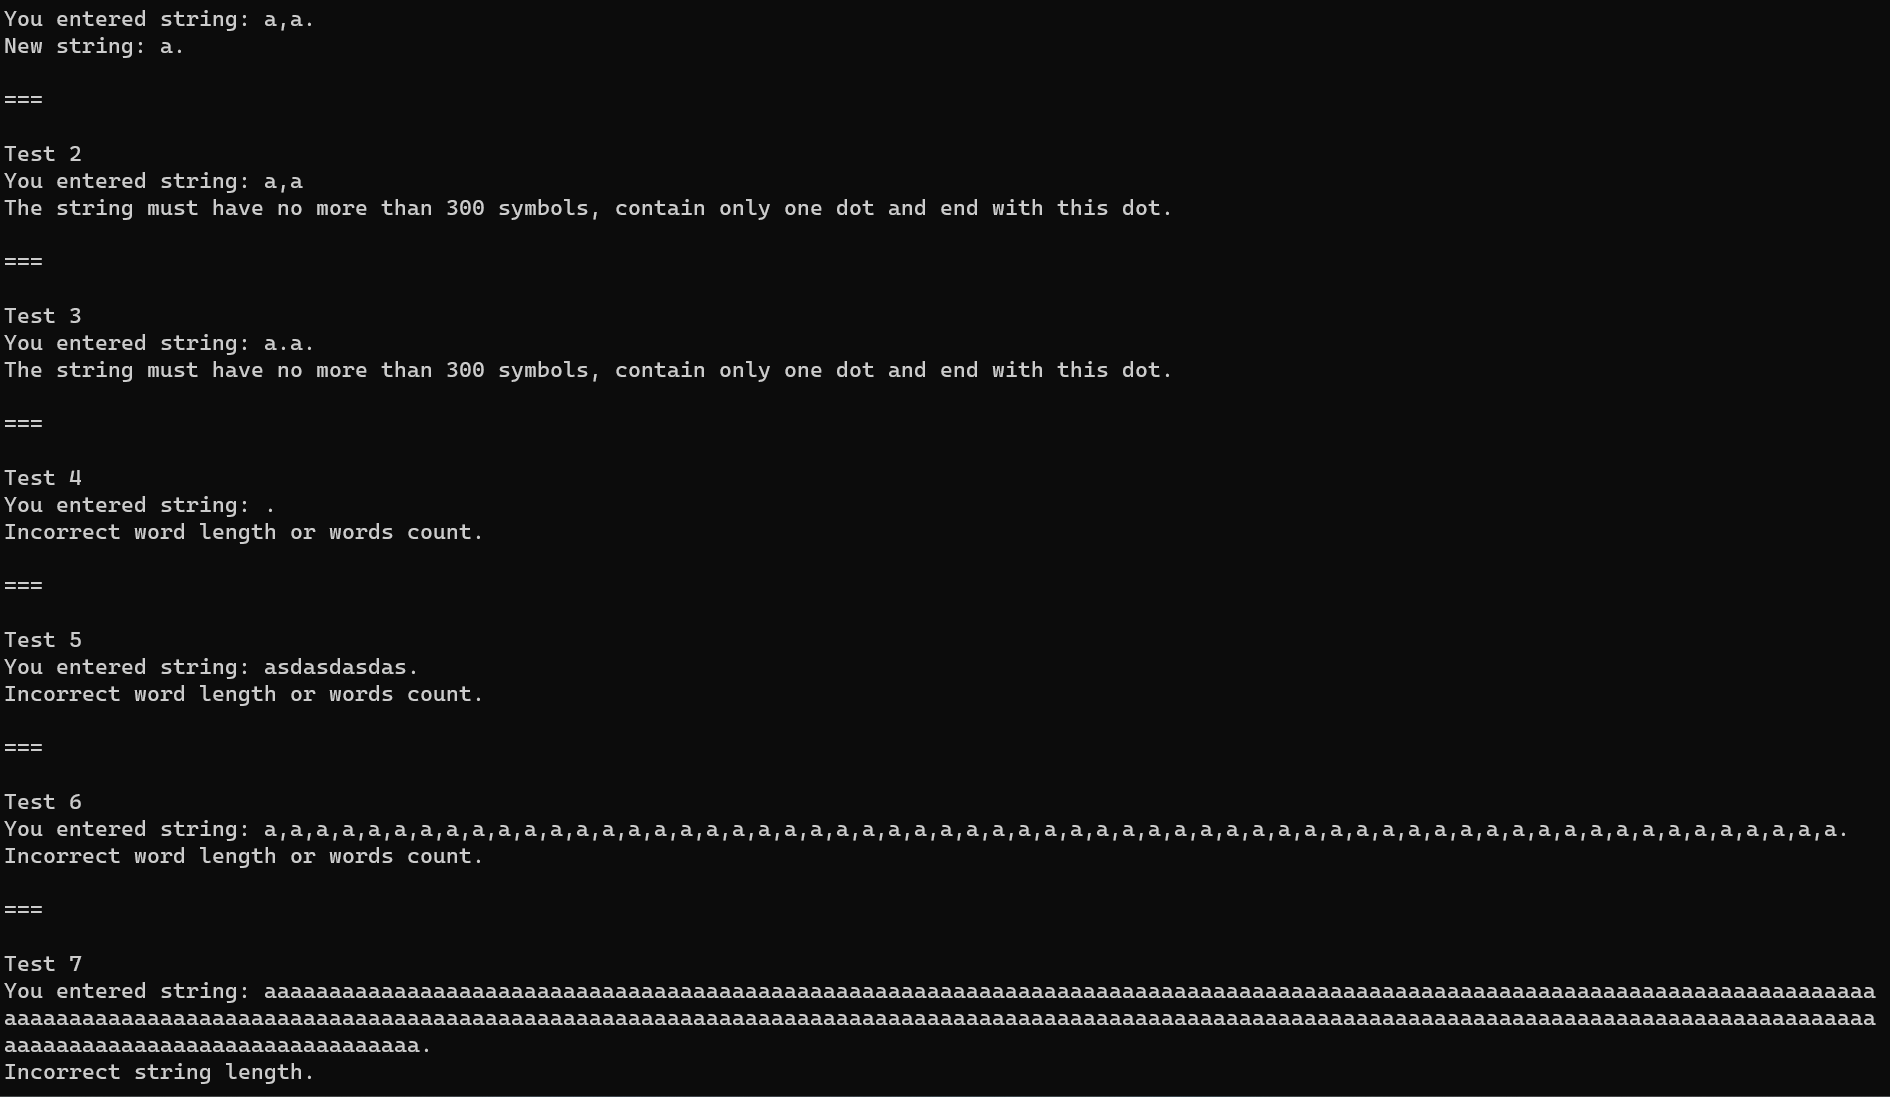
\includegraphics[width=400pt]{tests.png}
	
\end{document}
